%% bare_conf.tex
%% V1.3
%% 2007/01/11
%% by Michael Shell
%% See:
%% http://www.michaelshell.org/
%% for current contact information.
%%
%% This is a skeleton file demonstrating the use of IEEEtran.cls
%% (requires IEEEtran.cls version 1.7 or later) with an IEEE conference paper.
%%
%% Support sites:
%% http://www.michaelshell.org/tex/ieeetran/
%% http://www.ctan.org/tex-archive/macros/latex/contrib/IEEEtran/
%% and
%% http://www.ieee.org/

%%*************************************************************************
%% Legal Notice:
%% This code is offered as-is without any warranty either expressed or
%% implied; without even the implied warranty of MERCHANTABILITY or
%% FITNESS FOR A PARTICULAR PURPOSE! 
%% User assumes all risk.
%% In no event shall IEEE or any contributor to this code be liable for
%% any damages or losses, including, but not limited to, incidental,
%% consequential, or any other damages, resulting from the use or misuse
%% of any information contained here.
%%
%% All comments are the opinions of their respective authors and are not
%% necessarily endorsed by the IEEE.
%%
%% This work is distributed under the LaTeX Project Public License (LPPL)
%% ( http://www.latex-project.org/ ) version 1.3, and may be freely used,
%% distributed and modified. A copy of the LPPL, version 1.3, is included
%% in the base LaTeX documentation of all distributions of LaTeX released
%% 2003/12/01 or later.
%% Retain all contribution notices and credits.
%% ** Modified files should be clearly indicated as such, including  **
%% ** renaming them and changing author support contact information. **
%%
%% File list of work: IEEEtran.cls, IEEEtran_HOWTO.pdf, bare_adv.tex,
%%                    bare_conf.tex, bare_jrnl.tex, bare_jrnl_compsoc.tex
%%*************************************************************************

% *** Authors should verify (and, if needed, correct) their LaTeX system  ***
% *** with the testflow diagnostic prior to trusting their LaTeX platform ***
% *** with production work. IEEE's font choices can trigger bugs that do  ***
% *** not appear when using other class files.                            ***
% The testflow support page is at:
% http://www.michaelshell.org/tex/testflow/



% Note that the a4paper option is mainly intended so that authors in
% countries using A4 can easily print to A4 and see how their papers will
% look in print - the typesetting of the document will not typically be
% affected with changes in paper size (but the bottom and side margins will).
% Use the testflow package mentioned above to verify correct handling of
% both paper sizes by the user's LaTeX system.
%
% Also note that the "draftcls" or "draftclsnofoot", not "draft", option
% should be used if it is desired that the figures are to be displayed in
% draft mode.
%
\documentclass[10pt, a4paper, conference]{IEEEtran}
% \documentclass[draftcls,conference]{IEEEtran}
% Add the compsoc option for Computer Society conferences.
%
% If IEEEtran.cls has not been installed into the LaTeX system files,
% manually specify the path to it like:
% \documentclass[conference]{../sty/IEEEtran}





% Some very useful LaTeX packages include:
% (uncomment the ones you want to load)


% *** MISC UTILITY PACKAGES ***
%
%\usepackage{ifpdf}
% Heiko Oberdiek's ifpdf.sty is very useful if you need conditional
% compilation based on whether the output is pdf or dvi.
% usage:
% \ifpdf
%   % pdf code
% \else
%   % dvi code
% \fi
% The latest version of ifpdf.sty can be obtained from:
% http://www.ctan.org/tex-archive/macros/latex/contrib/oberdiek/
% Also, note that IEEEtran.cls V1.7 and later provides a builtin
% \ifCLASSINFOpdf conditional that works the same way.
% When switching from latex to pdflatex and vice-versa, the compiler may
% have to be run twice to clear warning/error messages.






% *** CITATION PACKAGES ***
%
\usepackage{cite}
% cite.sty was written by Donald Arseneau
% V1.6 and later of IEEEtran pre-defines the format of the cite.sty package
% \cite{} output to follow that of IEEE. Loading the cite package will
% result in citation numbers being automatically sorted and properly
% "compressed/ranged". e.g., [1], [9], [2], [7], [5], [6] without using
% cite.sty will become [1], [2], [5]--[7], [9] using cite.sty. cite.sty's
% \cite will automatically add leading space, if needed. Use cite.sty's
% noadjust option (cite.sty V3.8 and later) if you want to turn this off.
% cite.sty is already installed on most LaTeX systems. Be sure and use
% version 4.0 (2003-05-27) and later if using hyperref.sty. cite.sty does
% not currently provide for hyperlinked citations.
% The latest version can be obtained at:
% http://www.ctan.org/tex-archive/macros/latex/contrib/cite/
% The documentation is contained in the cite.sty file itself.






% *** GRAPHICS RELATED PACKAGES ***
%
\ifCLASSINFOpdf
  \usepackage[pdftex]{graphicx}
  % declare the path(s) where your graphic files are
  % \graphicspath{{../pdf/}{../jpeg/}}
  % and their extensions so you won't have to specify these with
  % every instance of \includegraphics
  % \DeclareGraphicsExtensions{.pdf,.jpeg,.png}
\else
  % or other class option (dvipsone, dvipdf, if not using dvips). graphicx
  % will default to the driver specified in the system graphics.cfg if no
  % driver is specified.
  \usepackage[dvips]{graphicx}
  % declare the path(s) where your graphic files are
  % \graphicspath{{../eps/}}
  % and their extensions so you won't have to specify these with
  % every instance of \includegraphics
  % \DeclareGraphicsExtensions{.eps}
\fi
% graphicx was written by David Carlisle and Sebastian Rahtz. It is
% required if you want graphics, photos, etc. graphicx.sty is already
% installed on most LaTeX systems. The latest version and documentation can
% be obtained at: 
% http://www.ctan.org/tex-archive/macros/latex/required/graphics/
% Another good source of documentation is "Using Imported Graphics in
% LaTeX2e" by Keith Reckdahl which can be found as epslatex.ps or
% epslatex.pdf at: http://www.ctan.org/tex-archive/info/
%
% latex, and pdflatex in dvi mode, support graphics in encapsulated
% postscript (.eps) format. pdflatex in pdf mode supports graphics
% in .pdf, .jpeg, .png and .mps (metapost) formats. Users should ensure
% that all non-photo figures use a vector format (.eps, .pdf, .mps) and
% not a bitmapped formats (.jpeg, .png). IEEE frowns on bitmapped formats
% which can result in "jaggedy"/blurry rendering of lines and letters as
% well as large increases in file sizes.
%
% You can find documentation about the pdfTeX application at:
% http://www.tug.org/applications/pdftex





% *** MATH PACKAGES ***
%
%\usepackage[cmex10]{amsmath}
% A popular package from the American Mathematical Society that provides
% many useful and powerful commands for dealing with mathematics. If using
% it, be sure to load this package with the cmex10 option to ensure that
% only type 1 fonts will utilized at all point sizes. Without this option,
% it is possible that some math symbols, particularly those within
% footnotes, will be rendered in bitmap form which will result in a
% document that can not be IEEE Xplore compliant!
%
% Also, note that the amsmath package sets \interdisplaylinepenalty to 10000
% thus preventing page breaks from occurring within multiline equations. Use:
%\interdisplaylinepenalty=2500
% after loading amsmath to restore such page breaks as IEEEtran.cls normally
% does. amsmath.sty thesisis already installed on most LaTeX systems. The latest
% version and documentation can be obtained at:
% http://www.ctan.org/tex-archive/macros/latex/required/amslatex/math/





% *** SPECIALIZED LIST PACKAGES ***
%
%\usepackage{algorithmic}
% algorithmic.sty was written by Peter Williams and Rogerio Brito.
% This package provides an algorithmic environment fo describing algorithms.
% You can use the algorithmic environment in-text or within a figure
% environment to provide for a floating algorithm. Do NOT use the algorithm
% floating environment provided by algorithm.sty (by the same authors) or
% algorithm2e.sty (by Christophe Fiorio) as IEEE does not use dedicated
% algorithm float types and packages that provide these will not provide
% correct IEEE style captions. The latest version and documentation of
% algorithmic.sty can be obtained at:
% http://www.ctan.org/tex-archive/macros/latex/contrib/algorithms/
% There is also a support site at:
% http://algorithms.berlios.de/index.html
% Also of interest may be the (relatively newer and more customizable)
% algorithmicx.sty package by Szasz Janos:
% http://www.ctan.org/tex-archive/macros/latex/contrib/algorithmicx/




% *** ALIGNMENT PACKAGES ***
%
%\usepackage{array}
% Frank Mittelbach's and David Carlisle's array.sty patches and improves
% the standard LaTeX2e array and tabular environments to provide better
% appearance and additional user controls. As the default LaTeX2e table
% generation code is lacking to the point of almost being broken with
% respect to the quality of the end results, all users are strongly
% advised to use an enhanced (at the very least that provided by array.sty)
% set of table tools. array.sty is already installed on most systems. The
% latest version and documentation can be obtained at:
% http://www.ctan.org/tex-archive/macros/latex/required/tools/


%\usepackage{mdwmath}
%\usepackage{mdwtab}
% Also highly recommended is Mark Wooding's extremely powerful MDW tools,
% especially mdwmath.sty and mdwtab.sty which are used to format equations
% and tables, respectively. The MDWtools set is already installed on most
% LaTeX systems. The lastest version and documentation is available at:
% http://www.ctan.org/tex-archive/macros/latex/contrib/mdwtools/


% IEEEtran contains the IEEEeqnarray family of commands that can be used to
% generate multiline equations as well as matrices, tables, etc., of high
% quality.


%\usepackage{eqparbothesisx}
% Also of notable interest is Scott Pakin's eqparbox package for creating
% (automatically sized) equal width boxes - aka "natural width parboxes".
% Available at:
% http://www.ctan.org/tex-archive/macros/latex/contrib/eqparbox/





% *** SUBFIGURE PACKAGES ***
%\usepackage[tight,footnotesize]{subfigure}
% subfigure.sty was written by Steven Douglas Cochran. This package makes it
% easy to put subfigures in your figures. e.g., "Figure 1a and 1b". For IEEE
% work, it is a good idea to load it with the tight package option to reduce
% the amount of white space around the subfigures. subfigure.sty is already
% installed on most LaTeX systems. The latest version and documentation can
% be obtained at:
% http://www.ctan.org/tex-archive/obsolete/macros/latex/contrib/subfigure/
% subfigure.sty has been superceeded by subfig.sty.



%\usepackage[caption=false]{caption}
%\usepackage[font=footnotesize]{subfig}
% subfig.sty, also written by Steven Douglas Cochran, is the modern
% replacement for subfigure.sty. However, subfig.sty requires and
% automatically loads Axel Sommerfeldt's caption.sty which will override
% IEEEtran.cls handlithesisng of captions and this will result in nonIEEE style
% figure/table captions. To prevent this problem, be sure and preload
% caption.sty with its "caption=false" package option. This is will preserve
% IEEEtran.cls handing of captions. Version 1.3 (2005/06/28) and later 
% (recommended due to many improvements over 1.2) of subfig.sty supports
% the caption=false option directly:
%\usepackage[caption=false,font=footnotesize]{subfig}
%
% The latest version and documentation can be obtained at:
% http://www.ctan.org/tex-archive/macros/latex/contrib/subfig/
% The latest version and documentation of caption.sty can be obtained at:
% http://www.ctan.org/tex-archive/macros/latex/contrib/caption/




% *** FLOAT PACKAGES ***
%
%\usepackage{fixltx2e}
% fixltx2e, the successor to the earlier fix2col.sty, was written by
% Frank Mittelbach and David Carlisle. This package corrects a few problems
% in the LaTeX2e kernel, the most notable of which is that in current
% LaTeX2e releases, the ordering of single and double column floats is not
% guaranteed to be preserved. Thus, an unpatched LaTeX2e can allow a
% single column figure to be placed prior to an earlier double column
% figure. The latest version and documentation can be found at:
% http://www.ctan.org/tex-archive/macros/latex/base/



%\usepackage{stfloats}
% stfloats.sty was written by Sigitas Tolusis. This package gives LaTeX2e
% the ability to do double column floats at the bottom of the page as well
% as the top. (e.g., "\begin{figure*}[!b]" is not normally possible in
% LaTeX2e). It also provides a command:
%\fnbelowfloat
% to enable the placement of footnotes below bottom floats (the standard
% LaTeX2e kernel puts them above bottom floats). This is an invasive package
% which rewrites many portions of the LaTeX2e float routines. It may not work
% with other packages that modify the LaTeX2e float routines. The latest
% version and documentation can be obtained at:
% http://www.ctan.org/tex-archive/macros/latex/contrib/sttools/
% Documentation is contained in the stfloats.sty comments as well as in the
% presfull.pdf file. Do not use the stfloats baselinefloat ability as IEEE
% does not allow \baselineskip to stretch. Authors submitting work to the
% IEEE should note that IEEE rarely uses double column equations and
% that authors should try to avoid such use. Do not be tempted to use the
% cuted.sty or midfloat.sty packages (also by Sigitas Tolusis) as IEEE does
% not format its papers in such ways.




% *** PDF, URL AND HYPERLINK PACKAGES ***
%
\usepackage{url}
% url.sty was written by Donald Arseneau. It provides better support for
% handling and breaking URLs. url.sty is already installed on most LaTeX
% systems. The latest version can be obtained at:
% http://www.ctan.org/tex-archive/macros/latex/contrib/misc/
% Read the url.sty source comments for usage information. Basically,
% \url{my_url_here}.


\usepackage{listings}
\usepackage{paralist}
\usepackage{color}
\usepackage{subcaption}

\usepackage{booktabs}
\usepackage{amssymb}
\usepackage{amsmath}
\usepackage{hyperref}
\usepackage{siunitx}
%\usepackage[disable]{todonotes}
\usepackage{todonotes}

\newcommand*\rot{\rotatebox{90}}
\newcommand*\rotninety{\rotatebox{90}}


\definecolor{mygreen}{rgb}{0,0.6,0}
\definecolor{mygray}{rgb}{0.5,0.5,0.5}
\definecolor{mymauve}{rgb}{0.58,0,0.82}
\definecolor{light-gray}{gray}{0.95}

\lstset{ %
  backgroundcolor=\color{white},   % choose the background color; you must add \usepackage{color} 
  basicstyle=\footnotesize\ttfamily,        % the size of the fonts that are used for the code
  breakatwhitespace=false,         % sets if automatic breaks should only happen at whitespace
  breaklines=true,                 % sets automatic line breaking
  captionpos=b,                    % sets the caption-position to bottom
  commentstyle=\color{mygreen},    % comment style
  frame=single,	                   % adds a frame around the code
  keepspaces=true,                 % keeps spaces in text, useful for keeping indentation of code (possibly needs columns=flexible)
  keywordstyle=\color{blue},       % keyword style
  numbers=left,                    % where to put the line-numbers; possible values are (none, left, right)
  numbersep=4pt,                   % how far the line-numbers are from the code
  numberstyle=\tiny\color{mygray}, % the style that is used for the line-numbers
  rulecolor=\color{black},         % if not set, the frame-color may be changed on line-breaks within not-black text (e.g. comments (green here))
  showspaces=false,                % show spaces everywhere adding particular underscores; it overrides 'showstringspaces'
  showstringspaces=false,          % underline spaces within strings only
  showtabs=false,                  % show tabs within strings adding particular underscores
  stepnumber=1,                    % the step between two line-numbers. If it's 1, each line will be numbered
  stringstyle=\color{mymauve},     % string literal style
  tabsize=2,	                   % sets default tabsize to 2 spaces
  title=\lstname                   % show the filename of files included with \lstinputlisting; also try caption instead of title
}


% *** Do not adjust lengths that control margins, column widths, etc. ***
% *** Do not use packages that alter fonts (such as pslatex).         ***
% There should be no need to do such things with IEEEtran.cls V1.6 and later.
% (Unless specifically asked to do so by the journal or conference you plan
% to submit to, of course. )


% correct bad hyphenation here
\hyphenation{op-tical net-works semi-conduc-tor DevOps}


% MAP dummy commands that are only used in the working template (e.g. to-dos)
\usepackage{xargs}
\newcommandx{\unsure}[2][1=]{}
\newcommandx{\change}[2][1=]{}
\newcommandx{\info}[2][1=]{}
\newcommandx{\improvement}[2][1=]{}
\newcommandx{\thiswillnotshow}[2][1=]{}

%\pdfpagewidth=8.5in
%\pdfpageheight=11in

\newcommand{\todomp}[1]{\todo[color=blue!20,inline]{\textbf{MP:} #1}}
\newcommand{\todoss}[1]{\todo[color=green!20,inline]{\textbf{Stefan:} #1}}
\newcommand{\todocontribution}{\todo[color=red!60,inline]{looking for contributions}}
\newcommand{\fmhkn}[1]{\todo[color=red!10,inline]{\textbf{HK
:} #1}}

%\usepackage{draftwatermark}
%\SetWatermarkText{Draft}
%\SetWatermarkScale{1}

\pagestyle{plain}
\begin{document}

% paper title
% can use linebreaks \\ within to get better formatting as desired

\title{AINFV: Analysis of Isolation (memory/packet) in Network Function Virtualization }
% 

%\author{\IEEEauthorblockN{Manuel Peuster}
%\IEEEauthorblockA{Paderborn University\\
%manuel.peuster@uni-paderborn.de}
%\and
%\IEEEauthorblockN{Holger Karl}
%\IEEEauthorblockA{Paderborn University\\
%  holger.karl@uni-paderborn.de}
%}

% author names and affiliations
\author{\IEEEauthorblockN{
    Abdul Ahad Ayaz\IEEEauthorrefmark{1},
  }
  \IEEEauthorblockA{\IEEEauthorrefmark{1}Paderborn University (ahad@mail.upb.de)
  }
  
}

% make the title area
\maketitle

\begin{abstract}
Network Function Virtualization (NFV) is a new way of defining a network with the help of software that was previously done with hardware middle-boxes. But there is isolation and performance overhead between NFV and hardware middle-boxes. The current approach is to run network function in either Virtual machine or Container, this ensures isolation but at the cost of performance degradation. In this seminar paper, NetBricks framework is discussed. This framework provides a new way of developing and running the network function. This paper further discussed isolation issues and performance overheads. A detailed comparison is provided between using the NetBricks framework and VMs/Containers.   
\end{abstract}



% For peer review papers, you can put extra information on the cover
% page as needed:
% \ifCLASSOPTIONpeerreview
% \begin{center} \bfseries EDICS Category: 3-BBND \end{center}
% \fi
%
% For peer review papers, this IEEEtran command inserts a page break and
% creates the second title. It will be ignored for other modes.
\IEEEpeerreviewmaketitle


\section{Introduction }
\label{sec:intro}

The starting days of networks, it was designed to send packets between two nodes. As the size of the network increased, technology evolved and many network services were introduced from time to time e.g. routing, forwarding, security, etc. Traditionally, these network services were deployed using hardware middleboxes i.e. firewall, routers, etc. These traditional hardware middleboxes are in the market for a very long time and still serving their purposes. But there are disadvantages of using this approach as mentioned in \cite{Philippov2017}: 
a) Inflexibility: unable to modify network services (proprietary issue); b) Non-Scalability: one needs to buy new middlebox if the load of network increases for a certain period of time and load stabilizes after some time then the new middlebox is useless; c) Cost: expensive in terms of upgrading the network components by replacing old middleboxes with latest middleboxes to get the maximum throughput. These disadvantages encouraged the European Telecommunication Standards Institute (ETSI)\cite{ETSI2012} in 2012 and the idea of Network Function Virtualization (NFV) was proposed. The idea was to replace the hardware middleboxes with software-defined network services and deploy these network services as Virtual Machine (VM) on commodity servers. ETSI proposed that NFV will help the service providers with swift deployment of network services comparatively cheap and more flexible. %As mentioned in \cite{Panda2017} NFV provides the blueprint of developing the network’s data plane, which allows the developer to program every packet forwarding in the network. Same in SDN (Software Defined Networking), which provides the blueprint of managing the control plane, i.e. allows a developer to define the custom routing, managing network failures, etc. 
NFV framework provides the following features\cite{Panda2017}:
\begin{itemize}
	\item Multiplexing: NFV framework should ensure that Network Functions (NF) should be hardware independent. This helps in scaling of NF without changing the hardware.
	\item Isolation: NF deployed in virtualized environment shares the underlying hardware. NFV framework should ensure the memory and packet isolation without affecting the performance. 
	\item High Performance: NF connected in series working as NF chains should have maximum throughput or equal to hardware middleboxes. NFV framework should ensure this throughput, as there is a major overhead of copying packets from one NF to others.
	\item Efficiency: Framework should ensure minimal hardware utilization as the aim of NFV is to utilize the commodity servers efficiently.
	\item Simplify NF Development: Framework should ensure the simplicity in development of NF, by separating the tasks into two categories i.e. user-defined functionality and pre-processing tasks. All of this should be automated. 
	\item Rapid Deployment: NFV Framework should ensure the rapid deployment by production ready NFs (e.g. NF testing and deployment in the production environment on the go, to improve the performance). This saves a lot of time.
\end{itemize}


NFV framework have many advantages but it is still long way from perfection in terms of development and deployment. For development part as addressed in \cite{Philippov2017} main issue is the performance trade-off due to low-level programming and optimization issues. No standard model is defined, thus every vendor has its programming model making NF operation complex to work in a multi-tenant network environment. For deployment, the current idea is to deploy NFs as VMs or Containers to ensure isolation as it is the main security concern. But at the cost of loss in performance loss. The main idea of this seminar paper is to ensure isolation without using VMs/Containers and deploy the NFs as a single process using NetBricks framework\cite{Panda2016} mentioned in section\ref{NetBricks}.
\section{Background}
%\subsection*{Requirements}
%As discussed earlier, NFV purpose is to simplify the development and deployment of NFs without changing the functionality and performance offered by traditional middleboxes. As mentioned in \cite{Panda2017}, some requirements must be fulfilled:
%\begin{itemize}
%	\item Performance: Framework should not take more than 10 seconds of a microsecond for processing packet. Single NF should be able to process 10-100Gbps of traffic. As the mentioned figures are equivalent to what we get with hardware middleboxes.  
%	\item Efficiency: Deployment should be done using a single machine because deployment across multiple machines will result in poor resource utilization and performance loss.
%	\item Chaining: Framework should be able to combine multiple NF called chaining i.e. NF1 to NF2...till NFn. Packet processing starts from NF1 to NFn. Fig.\ref{key1} shows the NF chain for processing web traffic.
%\begin{figure}
%	\centering
%	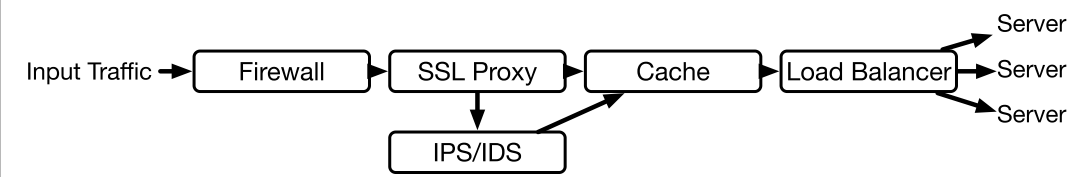
\includegraphics[width=\linewidth]{figures/fig1}
%	\caption{NF chain for serving web traffic\cite{Panda2017}}
%	
%	\label{key1}
%\end{figure}
%	\item Multi-vendor: NFV framework should support the multi-vendor NF to exists in a network, with security measures i.e. isolation.  
%	\item Multi-tenant: In the cloud environment multiple tenants exist, sharing the virtual resource provided by the service provider. NF should be deployed in such a way that the deployment for one tenant should not affect the operation of other tenants. 

%Mentioned requirements help in building well structured NFs and deployment ensuring the isolation. 
This section provides the background of traditional practices used for developing and deploying the NFs. To get the further insights, these practices are divided into development model, execution model and isolation.
%To get further insights into the NFV framework, NFV is divided into two parts, one part deals with the development model and the second part deals with the execution model.
%\end{itemize}
\subsection{Development Model}
Throughput and latency are two major metrics affecting network performance. Throughput is packet processing in a given time whereas latency is time between sending and receiving of a packet. These two metrics depend on the number of things \cite{Philippov2017}i.e. context switching, Translation Lookaside Buffer (TLB) misses and memory allocation. There are many libraries available for fast packet processing namely Data Plane Development Kit (DPDK)\cite{Corporation2014} and netmap etc. %As mentioned in \cite{Panda2017} DPDK libraries provide fast packet processing mechanism by a) Using PMD (Poll-mode Driver) instead of depending on the CPU interrupts for acknowledgment of received packet; b) assigning NIC (Network Interface Card) to single process instead of relying on kernel for NIC multiplexing; c) provides the interface for connecting NIC directly to NF, instead of using intermediate elements (i.e. vSwitch) that required additional computation for packet movement.
 These libraries help in improving performance and help developers to focus on optimization e.g. how the packets should be batched. 
 %The use of vectorization, as proposed in \cite{Philippov2017}, VPP (Vector Packet Processing) allows the processing on vectors of packets (i.e. up to 256 packets can be read at once.) 
As discussed in \cite{Panda2016}, The Click modular router \cite{Kohler2000} based on DPDK libraries provides the abstraction to develop new NF in such a way by combining multiple packet processing elements. But does not define the flow of packets between different elements. Click\cite{Martins2014} provides the limited functionality for customization. Hence for every new NF, developers have to re-write those elements from scratch, a lot of time is spent on optimizing the elements. 

Development model should be modular, some module with fixed functionality and common for all NFs, whereas other modules should be user-defined for specific functionality. A developer is responsible for optimizing the user-defined modules only.
\subsection{Execution Model}
Current practice is to deploy NFs in VMs or Containers and for communication vSwitch is used. VMs and Containers ensure the memory isolation i.e. operation on one NF will not affect the other NF in a network. vSwitch allows the NFs to periodically use the NIC for sending and receiving of packets in networks or between NFs. But all this processing of packets is just copying of packets in network and every NF has its copy of packets that violates the packet isolation i.e. at any point in time, only one NF should have access to that particular packet. VMs and Containers have  greater influence on performance degradation. As mentioned in \cite{Panda2016}, comparing single process of NetBricks with dedicated NIC, per-core throughput drops by 3x when processing 64B packets using Containers and up to 7x while using VMs. This performance degraded furthermore when NFs are chained, Containers are 7x slower compared to NF chained in a single process of NetBricks and VMs are up to 11x slower. Furthermore, NF chained single process is 6x faster than NF chained Containers or VMs, where each NF having its dedicated core. These results are further discussed in section\ref{isolation analysis} 
\subsection{Isolation}
Both packet and memory Isolation is the major challenge to achieve, as it directly affects the performance e.g. latency and throughput. The main reason for this performance gap is: Firstly during packet processing, packets tend to cross the memory isolation barrier. Secondly the use of context switch that ensures packet should cross core boundaries. These isolation issues can be catered as mentioned in \cite{Panda2016}: for memory isolation, instead of using VMs and Containers. Checks can be introduced both compile-time and run-time. For packet isolation, “Zero-Copy Software Isolation (ZCSI)” is proposed by the author in \cite{Panda2016} that ensures the “safe 0-copy” packet I/O between NFs. This is implemented using unique types\cite{Gordon}.

In order to address the issues of development and execution model, author proposed a framework called NetBricks\cite{Panda2016}. This framework showcased a different way of developing and executing network functions that contradict with the traditional approach. 

\section{NetBricks Framework}
\label{NetBricks}
\subsection*{Overview}
NetBricks, a framework for developing and executing NFs on a single machine. It requires the re-writing of NF compatible with NetBricks development model. As mentioned in \cite{Panda2016}, it is not a limitation because of two reasons: a) not enough development progress has been done for NFs; b) NetBricks can also co-exists with traditional NFs, at the cost of performance.
This framework provides both development and execution environment. For development model, it help developers to work on high-level abstraction of packet processing tasks and allows user-defined programmability. The execution model uses safe language and runtimes to ensure memory isolation, whereas the current approach i.e. VMs and Containers uses scheduling for isolation \cite{Panda2016}. Another important aspect to consider in execution model is communication between NFs. Message passing (inter-process communication) must not be modified by network function to ensure packet isolation. To achieve this functionality, NetBricks uses “static checks” to avoid packet copying. The author in \cite{Panda2016} named this functionality as "ZCSI". "ZCSI" allows achieving the memory and packet isolation as compared to VMs and Containers with no performance degradation. 

As discussed above, NetBricks is a complete package. In section below, development model is explained in detailed, later section describes the execution model to deploy the NFs.
\subsection{Main Components of Development Model}
 As described in \cite{Panda2016}, NetBricks allows developer to focus on the high-level programmability of network function. Network function programmability is divided into five sections: packet processing, bytestream processing, control flow, state management, and event scheduling.
\subsubsection{Packet Processing}
In NetBricks, packet structure consist of a) stack of header; b) the payload; c) reference to any per-packet metadata \cite{Panda2016}. The header contains a structure that defines the length of a packet based on functional computation of its contents. The payload is actual data carried by the packet. Metadata defines internal communication within NF and it is customizable by the developer using user-defined functions. These user-defined functions are passed along with header structure and can access last deciphered header along with payload and related metadata. The author provided the four packet operations as follows \cite{Panda2016}: 
\begin{itemize}

\item Parse: This operation takes the header type and structure as an input. Later analyzes the payload accordingly by using header type and update header stack. At the end header bytes are removed from the payload.

\item Deparse: This operation is applied on header stack, it removes the bottom header from stack and return it to payload. 
\item Transform:  This operation implements user-defined functions on header and payload, allows developer to modify the packet size i.e. by adding or removing bytes to payload as mentioned in “parse”. It also allows to add and modify the metadata of the packet. 
\item Filter: This operation is used to remove packets to be dropped at a specific node. It is a boolean operation return either True or False. Filter operation drops all the packets at specific node when the user-defined function returns the false value.
\end{itemize}
\subsubsection{Bytestream Processing}
Main function of bytestream processing is to convert bytes arrays into packets. User-defined functions are applied on the bytes arrays. In \cite{Panda2016}, author provided the two bytestream operations as follows: 
\begin{itemize}
\item Window: It takes four parameters as input i.e. window size, sliding increment, timeout, and stream user-defined function. Window is responsible for receiving and re-arranging the cached packets and create a stream. A user-defined function is called whenever there is enough data received to form a window of appropriate size, connection is closed or timeout expires. Window operation also forward all received packets without modifying them or drop all packets and generate the modified byte array using packetize \cite{Panda2016}. 
\item Packetize: It allows the conversion of byte arrays into packets. Providing byte arrays and header stack, packetize converts the data into packets and assign relevant header\cite{Panda2016}.
\end{itemize}
\subsubsection{Control Flow}
Control flow deals with branching required in NF chains. Branching is used to define the conditions i.e. re-routing the packets to specific port etc. Another purpose of branching is to move packets across cores for processing. To get the maximum performance, there should be minimum caching of data between cores. Control flow provides developer the abstraction for re-routing packets as desired e.g. by user-defined functions, port, address, etc. While implementing the NF chains, it allows the developer to select which packet should be routed to next NF. The author provides three operations for control flow \cite{Panda2016} as follows: 
\begin{itemize}
\item Group By: It allows the branching with-in NF and branching across NF chains. It takes two input: number of groups for packet re-routing and user-defined function returning the packets with the ID of a group to which it belongs.
\item Shuffle: This operation adds additional functionality to “Group By” operation i.e. branching is done based on cores. At “Runtime”, Group ID generated by shuffle is used to decide which core to be used for packet processing. Shuffle allows both user-defined and pre-defined grouping. 
\item Merge: This operation provides a junction, where all the different branches can be merged e.g. all packets from different branches entering a junction and exist as a single group.
\end{itemize}
\subsubsection{State Management}
When data is processed across multiple cores, performance degradation can be observed. Due to communication between core i.e. cache coherence etc. Typically, Developer program NF to partition state and avoid cross-core access or allow minimal access when required without using partition state. State management allows access across multiple cores. Within core accesses are synchronized but for cross-core accesses author proposed following options \cite{Panda2016}: a) No-external-access i.e. one core for each partition; b) Bounded inconsistency\cite{Panda2017} i.e. where one core has write access to partition and other cores only have read access; c) Strict consistency i.e. allows multi-read and multi-write access.

\subsubsection{Event Scheduling}
Event Scheduling allows the developer to create user-defined functions, that can be run repeatedly i.e. to monitor the NF and get the performance logs periodically, etc.
\subsection{Main Components of Execution Model}
NetBricks also provides the execution environment to run the NF. This model ensures isolation and also deals with NF placement and scheduling \cite{Panda2016}.
\subsubsection{Isolation}
\begin{itemize}
\item Memory Isolation: Traditionally, isolation is obtained by using VMs and Containers at the cost of performance loss for simple NF. Considering the complex NF, this performance loss dominates. In order to tackle this issue, NetBricks used a different approach to achieve isolation. It makes use of RUST \cite{TheRustTeam2016} safe language that ensures type checks and LLVM \cite{Lattner} as a runtime. This combination of safe language and runtime achieves the memory isolation similar to that is obtained using the hardware Memory Management Unit (MMU). As mentioned in \cite{Panda2016}, safe language and runtime ensures following: a) disallow pointer arithmetic; b) bound checking on array accesses i.e. preventing random memory accesses; c) disallow accesses to null object i.e. preventing undefined behavior to ensure memory isolation; d) type casts are safe. These above features can be achieved using high-level programming languages i.e. Java, C\#, etc, but these languages are not system friendly. 
\item Packet Isolation: The traditional mechanism is to send packets in a physical network, NFV follows the same footstep. NF send packets in the network by copying. This copying mechanism results in performance degradation of packet processing. NetBricks uses the unique types \cite{Gordon} instead of using the copying mechanism. As mentioned in \cite{Panda2016}, unique types are used to cater data races e.g. disallowing the simultaneous accesses to the same data. This approach is applied while implementing the NFs. When NF sends a packet, sender function losses the accesses to that packet and only relevant NF should have accesses to that packet. This ensures packet isolation without any copying of packets.
\end{itemize}

Above mentioned techniques used in NetBricks for isolation are referred to as ZCSI \cite{Panda2016}. NetBricks runs as a single process, packets are transferred between NFs using “function calls”. In case of NF chain, a queue is maintained at receiving end.
\subsubsection{Placement and Scheduling}
NetBricks operates as a single process in which many NFs can be run. Consider the NF chains running as a directed graph having access to multiple available NIC interfaces. Before implementing, NetBricks have to decide at which core NF chains should run. Based on this, NetBricks make the scheduling decisions for packet processing. As the author mentioned in \cite{Panda2016}, currently NetBricks places all the network functions on a single core to get the maximum performance. In case of complex placements, NetBricks use "shuffle" operation to process packets across multiple cores. 
In \cite{Panda2016}, author uses the “run-to-completion” scheduling for NetBricks i.e. packets entering NF, it starts processing till it exists. Scheduling is needed when dealing with more than one packet, considering this all packets are added to  “window” and “group by” operation. NetBricks uses “round-robin” scheduling for these operations. 
%\subsection{Testing}
%To test and validate the NetBricks, two network functions were re-programmed \cite{Panda2016}. Firstly, the NF that decrements the IP TTL (Time To Live) and drops the packet with TTL zero. Secondly, google’s Maglev\cite{Yaghoubi2012} (i.e. load balancer).
 
%For the first example network function is build using NetBricks as shown in fig. \ref{key2}. Network functions are described as a public function in the RUST module. Line 1 of fig.\ref{key2} shows how the new instance of network function is created using the “ttl\_nf” function. During the network function processing, at line 3 ethernet (MAC) header is parsed from the packet and later at line 4 IP header is parsed from the packet. “Transform” operation is applied on the parsed IP header decrementing the packet’s TTL (line 5). After the computation of packet’s TTL, “Filter” operation is performed that drops the packets having TTL zero (line 9). In the end “Compose” operation at line 12 indicate the end of the description of network function and also allows the chaining of network function. As shown in fig.\ref{key2}, no “Shuffle” operation is applied while defining the network function. By default, NetBricks routes all the packet processing to a single core. Fig.\ref{key3} shows the code that is used to execute the user-defined functions. “NetbricksContext” is used to execute the user configuration. As mentioned in \cite{Panda2016}, at line 4 pipeline is created that : a) receives packets from input queue; b) these packets are forwarded to network function i.e. “ttl\_nf” for processing; c) later processed packets are again to the same queue. Placement of the pipeline is defined in user configuration.
%\begin{figure}
%	\centering
%	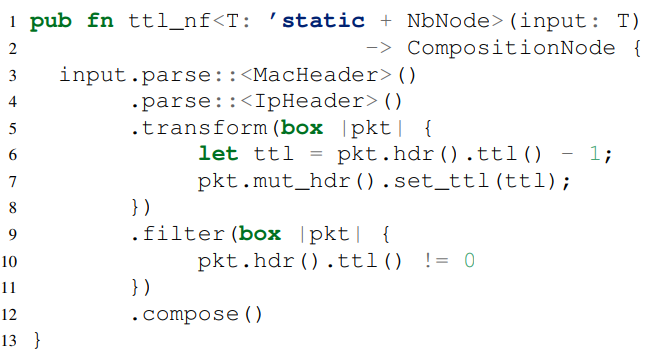
\includegraphics[width=\linewidth]{figures/fig2}
%	\caption{NetBricks code for Example NF\cite{Panda2016}}
%	
%	\label{key2}
%\end{figure}
%\begin{figure}
%	\centering
%	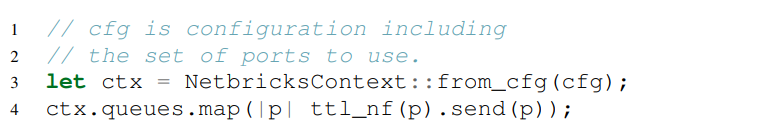
\includegraphics[width=\linewidth]{figures/fig3}
%	\caption{NetBricks code for Executing Example NF\cite{Panda2016}}
%	
%	\label{key3}
%\end{figure}

%For the second example, the author used load balancer (Maglev) network function and tried to implement it using NetBricks. Maglev is responsible for dividing the user requests among the back-end servers. Maglev ensures that it can be deployed in a replicated cluster for scalability and fault tolerance, splits traffic and handles failures. Maglev uses a hashing algorithm (i.e. based on a lookup table) to achieve the aims mentioned above \cite{Panda2016}. Fig.\ref{key4} shows the packet processing and forwarding part of Maglev.  First, the lookup table is created (line 8) and then a cache for recording the backend (line12) that is used to start the instance of Maglev network function. Starting at line 15, the network function is declared. Second, the “Shuffle” operation (line 16) uses the built-in functionality of using a single core. At line 17 ethernet headers are being parsed. Later  “Group by” operation (line18) is performed, it uses the “ipv4\_flow\_hash” built-in function to extract the flow hash i.e. consist of IP header and TCP or UDP header. This hash is used for two purposes: a) ensuring that the received packet is TCP or UDP ; b) to find the already assigned backend to flow (line 24) or to assign new backend to flow using a lookup table (line 25). In the end, network functions generate the vector of nodes relevant to the backend, specified by the operation.
%\begin{figure}
%	\centering
%	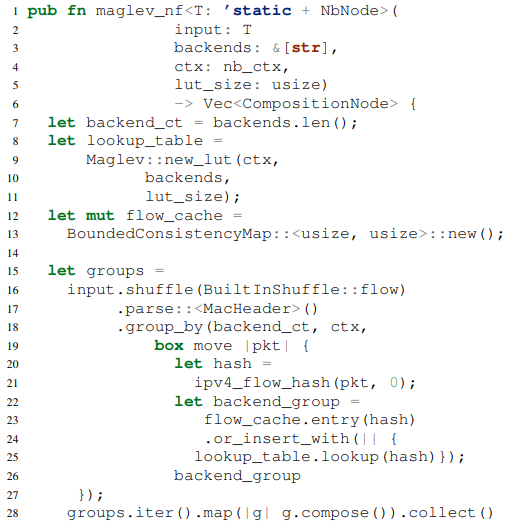
\includegraphics[width=\linewidth]{figures/fig4}
%	\caption{NetBricks code for google Magvel\cite{Panda2016}}
%	\label{key4}
%\end{figure}   
%\subsection{Analysis Tool}
%NetBricks network function chains are build using RUST language and mechanism proposed by the author. That is in contradiction with currently available frameworks i.e. OpenMANO etc. These frameworks provide the developer with an interface to manage without knowing the underlying programmability used for building the network functions. Author in \cite{Panda2016} also proposed to use the same interface, as it provides the following advantages: a) provides many optimization opportunities, currently using the RUST compiler’s optimization for optimizing the chaining code, later LLVM’s link-time optimization \cite{Lattner} can be used to optimize the whole program, improving performance of packet processing; b) it can be used to execute the complex network function chains and branches.
\section{Framework Evaluation}
This sections describes about the overheads of NFs developed using NetBricks compared to baseline NF build using other frameworks that was deployed on a testbed with specification mentioned in \cite{Panda2016}. Furthermore it presents the performance and isolation analysis of NetBricks NF comapared to NF build with other frameworks.
%\subsection{Testbed}
%For evaluating the NetBricks, as mentioned in a \cite{Panda2016} testbed with the following configuration was used: dual-socket servers with Intel Xeon E5-2660 2.6GHz CPUs, each having 10 cores. Each having 120GB of RAM, divided between sockets. Each server was also equipped with Intel XL710 QDA2 40Gb NIC. Hyper-threading was disabled and hardware virtualization was enabled i.e. Intel VT. Servers running Linux kernel 4.6.0-1 and DPDK 16.04 and programming language RUST nightly version. Two virtual switches were used i.e. first Open Vswitch with DPDK (OVS DPDK) \cite{Gross2014} and second SoftNIC \cite{Han:EECS-2015-155}. VMs used were running on KVM connected to a virtual switch with DPDK’s “vhost-user” driver. As per the requirement of DPDK, Docker containers were used with privileged mode and for their connection to a virtual switch, DPDK’s ring PMD driver was used. By default, PMD driver does not allow both virtual switches to copy packets and no packet isolation was observed as network function can modify the packets after they sent it. To achieve isolation the author made few modifications in virtual switches, allowing copying while connecting to containers. Even this copying using DPDK’s PMD driver has higher performance than other approaches i.e. “veth” pair. To test the traffic, the DPDK-based packet generator was used running on a separate server having 40Gb NIC. This server was directly connected to the test server without any intermediate switches. This packet generator server acted as a source and sink. Performance (i.e. throughput and latency) results were collected at the sink.

\subsection{Overheads and Results}
This section describes the development model overheads imposed by the NetBricks and the results obtained. For comparison purposes, both NIC and DPDK were configured the same for NetBricks and baseline NF. In \cite{Panda2016}, the author mentioned few overheads that are as follows: a) for simple NF; b) for checking array bounds.

In the case of simple NF, the packet TTL NF was used. This NF decrements the time-to-live (TTL) parameter of packet upon receiving packets and drops the packet with TTL equal to zero. Both NetBricks version and normal version of NF were executed using a single core by send packets of 64 bytes and observed the throughput. The result of both NFs were almost the same as expected by the author. As mentioned in \cite{Panda2016}, after 10 experimental runs, the average throughput observed for baseline NF was 23.3 million packets per second (MPPS) whereas for NetBricks NF it was observed 23.2 MPPS. For latency at 80\%, the round trip time (RTT) for baseline NF observed was \SI{16.15}{\micro\second} compared to NetBricks NF that was \SI{16.16}{\micro\second}.

\begin{figure}
	\centering
	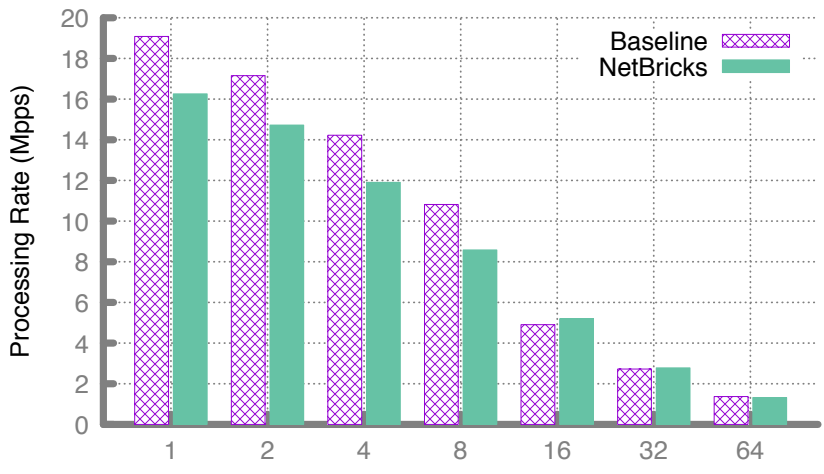
\includegraphics[width=65mm]{figures/fig5}
	\caption{Throughput comparison between NetBricks NF and Basline NF\cite{Panda2016}}
	
	\label{key5}
\end{figure}

In the case of array accesses \cite{Panda2016}, the safe language was used that imposed some overheads i.e. array bound checking. These checks can be a major source of the overhead of safe language i.e. Null-checks and other safety checks performed at runtime are difficult to separate. To test these checks overhead, NF was used that updates several cells in a 512KB array during packet processing\cite{Panda2016}. The update of these array cells depends on a UDP source port number of packet under processing, making it difficult to ignore array bound checks. The author compared the NetBricks NF with baseline NF executed using single-core and used packets with random UDP source port\cite{Panda2016}. Fig.\ref{key5} shows the throughput achieved by two NFs when memory accesses per packet increased. NetBrick’s throughput was 20\% less as compared to the baseline NF for 1 to 8 memory accesses. As the number of accesses increased i.e. 16 or more, the effect of checks overhead started to fade out\cite{Panda2016}. This is because of large memory accesses causing cache misses resulting in reduced throughput. These cache misses dominating the overhead imposed by the NetBricks. Array bound checking is an overhead of NetBricks resulting in less throughput.    


\subsection{Performance analysis of framework based different NFs}
To further validate the development model of NetBricks, author implemented different categories of network functions using the NetBricks framework. Some of them are mentioned below\cite{Panda2016}:
\begin{itemize}
\item Firewall: Based on Click \cite{Martins2014}, performs the linear scan of an Access Control List (ACL) to find relevant entry.
\item NAT: Based on MazuNAT [], Network Address Translation (NAT) built using Click.
\item IDS: Based on Snort \cite{Roesch}, for signature matching.
\item Monitor: Maintains per-flow counter similar to monitor module of Click.
\item Load balancer: based on Maglev\cite{Yaghoubi2012} , load balancer used by google.
\end{itemize}
\begin{figure}
	\centering
	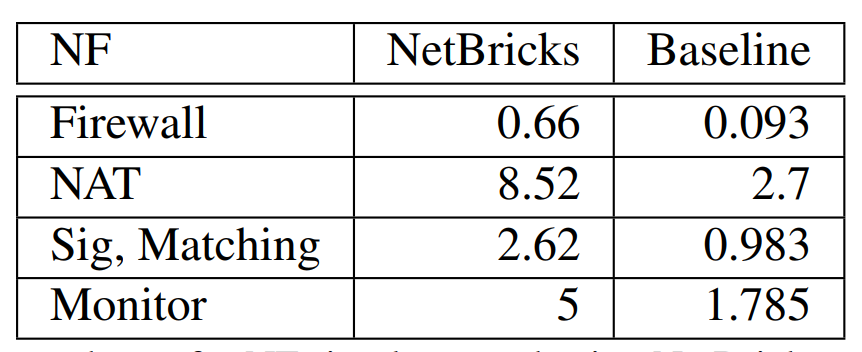
\includegraphics[width=70mm]{figures/tab1}
	\caption{Performance figures of NetBricks NF w.r.t other NFs\cite{Panda2016}}
	
	\label{key6}
\end{figure}

Testing of the above-mentioned NFs were performed using both NetBricks framework and original NF. These NFs were executed on a single core\cite{Panda2016}. Comparison results can be seen in fig.\ref{key6}, NetBricks NF performance is better as compared to other framework NF. As mentioned in \cite{Panda2016}, NetBricks NAT has a 3x better performance than MazuNAT. 

Further experiments were performed on the NetBricks version of Maglev. This testing were on multi-core\cite{Panda2016}. Fig.\ref{key7} show the comparison of NetBricks version of Maglev with google Maglev. It was observed that NetBricks throughput (MPPS) is  2.9x to 3.5x better compared to results mentioned in \cite{Yaghoubi2012}. Average latency observed was \SI{19.9}{\micro\second} for NetBricks and \SI{32}{\micro\second} for the original Maglev. These throughput and latency results are better but not to rely on because these two experiments (i.e. NetBricks Maglev version and Google Maglev) were performed on two different test-bed\cite{Panda2016}.    
\begin{figure}
	\centering
	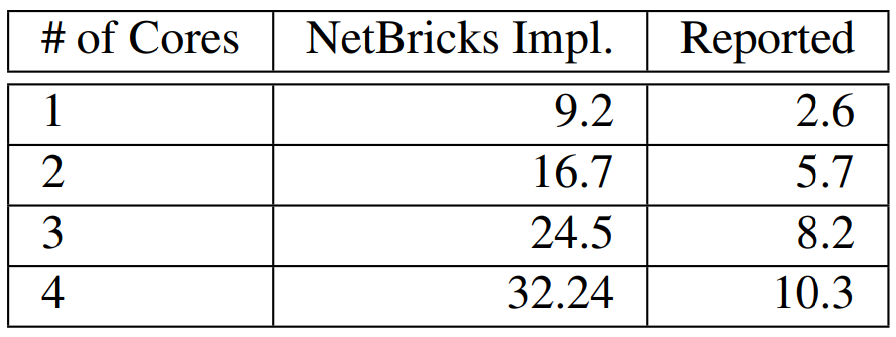
\includegraphics[width=70mm]{figures/tab2}
	\caption{Throughput (MPPS) achieved comparing NetBricks Multi-core with Maglev\cite{Panda2016}}
	
	\label{key7}
\end{figure}
\subsection{Isolation Analysis}
\label{isolation analysis}
This section discussed about the isolation achieved using the NetBricks isolation model.Isolation is ensured by NetBricks using safe language and runtime checks to avoid costs associated with core boundaries and crossing process \cite{Panda2016}. The author first checked the cost involved with the single NF. Evaluation was done to check the results when the length of the packet TTL NF chain increases. One point to consider here is that these costs are only applicable for simple NFs, but when the computational cost of NF is higher then NetBricks execution environment becomes irrelevant\cite{Panda2016}.
\subsection*{NF vs NF Chains vs Complex NF}
\begin{figure}
	\centering
	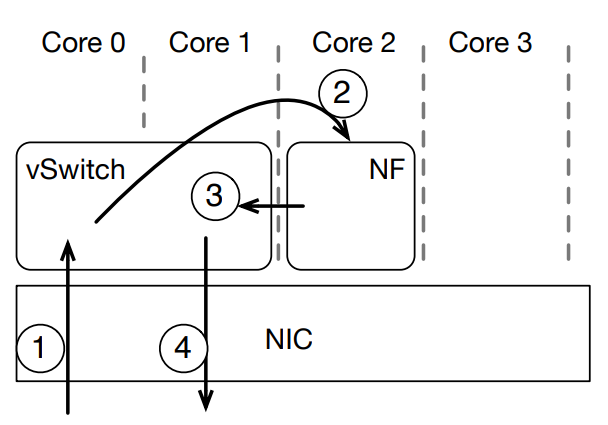
\includegraphics[width=65mm]{figures/fig6}
	\caption{VM/Container execution environment for simple NF\cite{Panda2016}}
	
	\label{key8}
\end{figure}
\begin{figure}
	\centering
	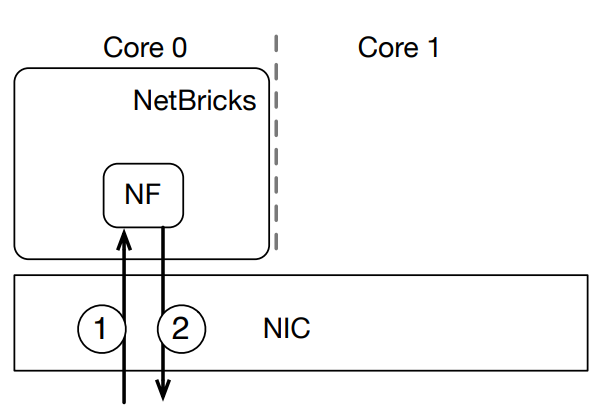
\includegraphics[width=65mm]{figures/fig7}
	\caption{NetBricks execution environment for simple NF\cite{Panda2016}}
	
	\label{key9}
\end{figure}
\begin{figure}
	\centering
	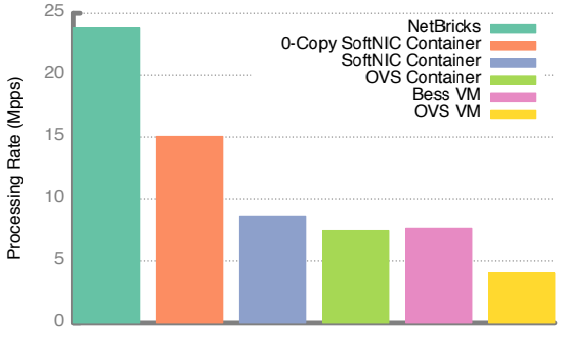
\includegraphics[width=65mm]{figures/fig8}
	\caption{Throughput achieved using different isolation techniques\cite{Panda2016}}
	
	\label{key10}
\end{figure}
This section presents the analysis of single NF, NF chain and complex NF in term of isolation and for that author compared the NetBricks with VMs or Containers \cite{Panda2016}. 

First case, single NF “that swaps the source and destination ethernet address for received packets and forward them out the same port” \cite{Panda2016} was built using NetBricks. The other NF was built using C language were compared and executed in their execution environment i.e. VM, Container, and NetBricks. Fig.\ref{key8} shows the test environment of VM and Container. A vSwitch was used that receives packets from NIC and forward them to network function running in either VM or Container. NF process those packets and forward them back to vSwitch, which was then forwarded to NIC. Both vSwitch and NF was running on DPDK and depend upon polling\cite{Panda2016}. For better performance NF was assigned its dedicated CPU and two cores were assigned to vSwitch. As mentioned in \cite{Panda2016}, with isolation comes two kinds of overheads: first due to cache and context switching cost i.e. cost associated with cross process or crossing core boundaries. Second due to packets copying. To analyze these isolation overheads, the author used SoftNIC to send packets between Containers without copying i.e. 0-copy SoftNIC Container violating packet isolation, later compared it with NetBricks\cite{Panda2016}. As shown in fig.\ref{key9}, NetBricks receives packets directly from NIC, process them using NF code and send them back to NIC, all this process was running on single-core. Fig.\ref{key10} shows the throughput achieved by different isolation techniques. As discussed in \cite{Panda2016}, Comparison of 0-copy SoftNIC Container with NetBricks with respect to throughput shows that 0-copy SoftNIC Container is 1.6x slower then NetBricks due to crossing core boundaries. Even though NetBricks was running on single-core and other was using three cores for processing. SoftNIC Container is 2.7x slower than NetBricks due to packet copying. This performance further degrades when using VM instead of Containers. Because VM uses the “vhost\_user” communication channel developed by DPDK from interacting with VM has more performance issues as compared to DPDK’s ring PMD driver used for Container\cite{Panda2016}.
\begin{figure}
	\centering
	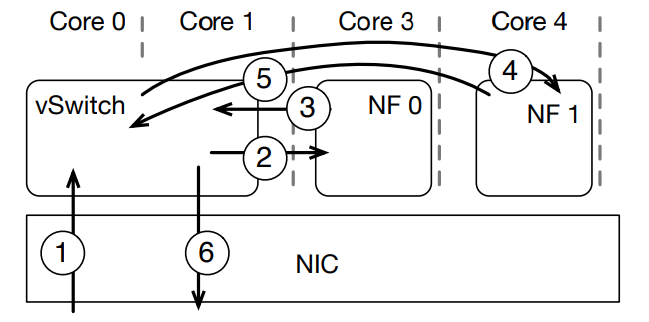
\includegraphics[width=65mm]{figures/fig9}
	\caption{VM/Container Execution environemt for NF chain\cite{Panda2016}}
	
	\label{key11}
\end{figure}
\begin{figure}
	\centering
	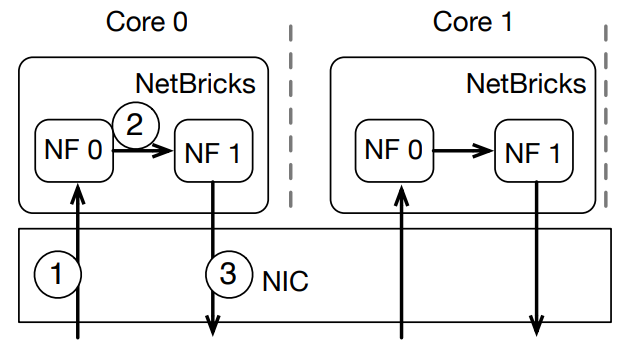
\includegraphics[width=65mm]{figures/fig10}
	\caption{NetBricks Execution environemt for NF chain\cite{Panda2016}}
	\label{key12}
\end{figure}

Second Case, NF chain i.e. multiple instances of single NF, compute packet’s TTL  and drops the packet with TTL 0\cite{Panda2016}. Fig.\ref{key11} shows the execution environment using VM or Container to run the network function chain e.g. NF0 and NF1. Author assigned two cores to vSwitch and two cores for NF chain, one for each NF. Fig.\ref{key12} shows the execution environment of NetBricks to run the NF chain e.g. NF0 and NF1. NetBricks was tested for two cases\cite{Panda2016}: a) with single-core; b) with two-cores. Fig.\ref{key13} shows the throughput comparison of NetBricks with single-core, multi-core, VM and Container. As mentioned in \cite{Panda2016}, NetBricks multi-core (NB-MC) is 7x better than a container with SoftNIC and 11x better compared to VM with SoftNIC\cite{Panda2016}. NetBricks with single-core (NB-SC) is 4x better than a container with SoftNIC and 6x better compared to VM with SoftNIC\cite{Panda2016}. The author also compared the 0-copy SoftNIC container and observed that with a packet size of 64 Bytes, it resulted in 3x times performance loss. As shown in fig.\ref{key13}, NetBricks multi-core throughput decreased when the size of the chain increased from 4. The author explained this decrease in throughput is due to more cores tries to accesses the NIC (i.e. 4 parallel I/O threads)\cite{Panda2016}. Above throughput figures are for a packet size of 64 Bytes. Increasing the packet size degrades the performance by 15\% \cite{Panda2016}. Fig.\ref{key14} shows the latency when using different isolation techniques.
\begin{figure}
	\centering
	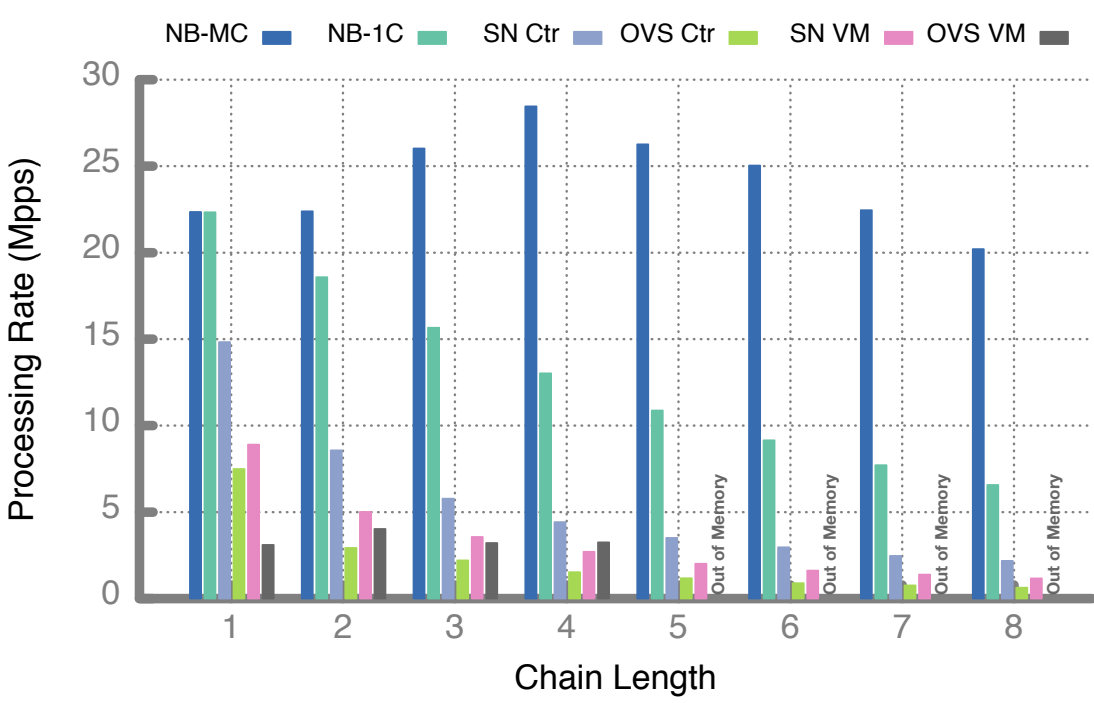
\includegraphics[width=65mm]{figures/fig11}
	\caption{Throughput of increasing NF chain, NetBricks single and multi core vs other technologies\cite{Panda2016}}
	\label{key13}
\end{figure}

Third case, complex NF i.e. increases computation cycles for per-packet processing and used the same execution environment as the first case fig.\ref{key8} and \ref{key9} as mentioned in \cite{Panda2016}. Three core were assigned for VM and Container i.e. one for NF and two for vSwitch and in case of NetBriciks two cases were tested\cite{Panda2016}: single-core and three-cores. The author modified the NF to use busy loops for the number of cycles after packet processing. Fig.\ref{key14} shows the throughput comparison of per-packet processing by using different isolation techniques. As mentioned in \cite{Panda2016}, increasing complexity of network function results in increased computation time that overcomes the improvements offered by NetBricks e.g. 300 cycles per packet. As shown in fig.\ref{key15}, NetBricks isolation performs better as compared to other techniques e.g. VM or Container. NetBricks multi-core throughput is 4x better as compared to other technologies when complexity level is low e.g. 100 cycles per packet. As the complexity increase upto 600 cycles per packet, NetBricks mutli-core still performs as better as 2x comapred to VM and Containers.  
\begin{figure}
	\centering
	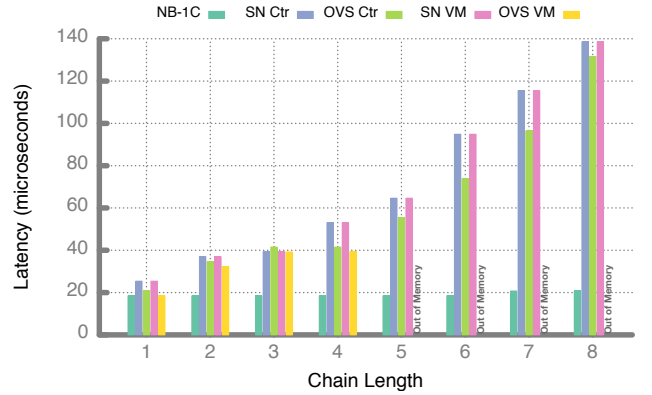
\includegraphics[width=65mm]{figures/fig12}
	\caption{Latency for increasing NF chain, NetBricks single/multi-core vs other technologies\cite{Panda2016}}
	\label{key14}
\end{figure}
\begin{figure}
	\centering
	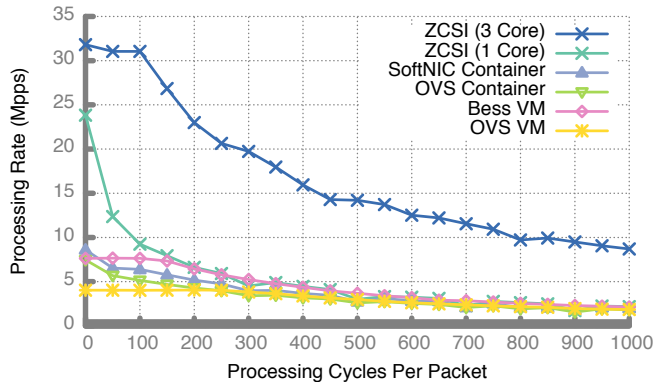
\includegraphics[width=65mm]{figures/fig13}
	\caption{Throughput of Complex NF using different isolation techniques\cite{Panda2016}}
	\label{key15}
\end{figure}
\section{Comparison of Frameworks}
In this section, NetBricks is compared with other frameworks available in the market. This comparison is done based on the development model, execution model, and isolation.
\subsection{Development Model}
In terms of development model, there are many frameworks available such as YANFF\cite{Philippov2017} that helps in rapid NF development. It is based on DPDK and uses GO language that is high-level, safe with built-in support for concurrency. YANFF uses the scheduler for packet processing across multiple cores, whereas in NetBricks it is done by explicit “shuffle” operations. YANFF has no dependencies on the execution environment. Next is libVNF\cite{Naik2017}, a reusable library for developing high performance and scalable NFs. An API is used, that provides the high-level abstraction and manages low-level optimization. It separates the application-specific processing of NFs from the software stack that can be reusable or common for all NFs. Compared to NetBricks, libVNF supports clustered NFs deployment and horizontal scalability i.e. ensuring high availability. FLICK \cite{Abdul} framework is used for development and deployment of NF. FLICK structure is quite similar to NetBricks, both use their own programming languages for development and have their own execution environment to run the developed NF. FLICK language allows to focus on only application-specific logic ignoring low-level details. Developed NF is compiled using the FLICK compiler that converts the FLICK program into C++, which is then compiled and linked with FLICK runtime for execution.
\subsection{Execution Model}
In terms of the execution model, NetVM \cite{Hwang2015} is a virtualization-based platform that uses shared memory to exploit the DPDK library i.e. ensuring 0-copy between VMs. It uses the hypervisor-based switch to control the flow of packets and inter-VM communication. Also ensure isolation to some extent e.g. packet accesses to only trusted VMs. OpenNetVM\cite{Yurchenko2018} is based on the NetVM framework, it uses Docker Container instead of VM. OpenNetVM consists of two main components: first, NF Manager that interact with NICs and responsible for packet flow management and inter-container communication. Second NFlib API that is used to connect NF i.e. container to NF Manager. It also allows the development of user-defined NF and makes use of NFlib to connect with NF Manager. HyperNF \cite{Yasukata2017} is VM based framework, fully utilizing the available resources e.g. CPU cores. No dedicated cores assigned for packet I/O as per the merge model mentioned in \cite{Yasukata2017} and packet I/O are part of VM. It uses “hypercall” instead of packet forwarding and communication between VMs. Compared to NetBricks, HyperNF is based on standard NFV architecture whereas NetBricks completely rewrites the software middleboxes. G-NET \cite{Zhang2018} framework is based on GPU-virtualization. It consists of three main components: “Switch” is a virtual switch for packet I/O and forwarding packets between network functions; “Manager” is proxy for GPU, it receives a request from network function for GPU computation; “Scheduler” is used for GPU resource allocation. G-NET also ensure the data isolation by using “isoPointer”.
\subsection{Isolation}
In terms of Isolation, SafeBricks \cite{Poddar2018} framework is based on NetBricks with some modifications. It is more oriented to cloud security. It ensures only encrypted traffic is exposed to the cloud. SafeBricks used the concept of “hardware enclave” using Intel SGX i.e. ensures that software even kernel or hypervisor outside the enclave cannot tamper with enclave. It allows the NF to run inside the enclave and in the cloud, it seems like a black box. Fig.\ref{key16} shows the author’s comparison of the different framework (i.e. xOMB\cite{Anderson2012}, CoMB\cite{Sekar}, ClickOS\cite{Martins2014}, HyperSwitch\cite{Ram2013}, mSwitch\cite{Honda2015}) in context with isolation.
\begin{figure}
	\centering
	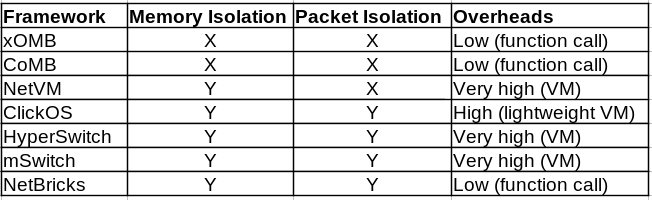
\includegraphics[width=65mm]{figures/fig14}
	\caption{Isolation between different frameworks\cite{Panda2016}}
	\label{key16}
\end{figure}
\section{Conclusion}
This seminar paper presented the detailed analysis of isolation. Current approaches e.g. VMs and Container ensures isolation but at the cost of performance degradation. This performance loss encouraged the entry of NetBricks. NetBricks contradicts with the current approaches. It runs the NF as a single process and for isolation it uses Type checking, array bound checking and unique types. The results mentioned in this paper shows that NetBricks performance is far better as compared to current approaches while ensuring the isolation.
\section{Further Research Topics}
 Optimation of RUST language to remove the overhead of the NetBricks framework. Currently, it supports multi-core processing, but further optimizations can be done to get even better throughput. Currently, NetBricks works on the data plane and control plane functionality can be added in the future to get better performance. Lastly, the current approaches integrates with MANO systems for management and Orchestration of NFs. NetBricks should also support MANO systems to compete in the market.
\label{sec:conclusion}




\bibliographystyle{IEEEtran}
\bibliography{IEEEabrv,main}

% that's all folks
\end{document}
